\section{文献相关程度与可比范围}
\label{sec:evidence-distance}

\subsection{分类依据}

本文按研究对象与目标相的关系组织文献，不将整篇论文简单归入单一类别。同一研究可分别为结构、合成路线或表征方法提供依据，每条结论仅适用于该文献直接观察的对象。文献分为五类：目标化合物的直接报道、无Zn的同类Ba--Y四方硅酸盐、具有明确晶体学关系的结构相关化合物、可作工艺参照的合成研究，以及不能支持目标结构或配方判断的非相关资料。分类用于说明结论的适用范围，不评价论文质量。

\paragraph{目标化合物的直接报道。}化学式须与$\mathrm{Ba_5Y_{12}Zn[O(SiO_4)]_8}$一致，且原始研究须同时给出制备过程和结构鉴定。目前仅Ababaikeri等报道的开放体系高温溶液法生长与单晶X射线结构研究符合这一条件\cite{ababaikeri2024ba5y12zn}。该研究提供了唯一的直接实验起点，但尚未建立可独立复现的块体相纯窗口。

\paragraph{同类Ba--Y四方硅酸盐。}此类研究不含Zn，但直接涉及四方Ba--Y硅酸盐的历史命名、结构重新审定或相区关系。早期工作报道了暂定的$\mathrm{Ba_{5+x}Y_{13}Si_8O_{41}}$伴生相\cite{kolitsch2009crystal}；现代单晶研究将相关组成重新审定为非化学计量调制结构\cite{yamane2024synthesis}；独立研究则以多种衍射和成分分析方法确认了四方$\mathrm{Ba_5Y_{13}[SiO_4]_8O_{8.5}}$\CJKecglue{}\cite{gulay2024navigation}。这些结果可限定历史化学式、组成范围和竞争相，但不能替代含Zn目标相的复现。

\paragraph{结构相关化合物、工艺参照与非相关资料。}具有可靠晶体学数据的Ba--Zn--Si--O或Ba--Y--Si--O化合物，可用于比较多面体连接方式、阳离子位点和相变表征\cite{liu1993structures,lin1999phase,zou2021crystal,motozawa2022bay16si4o33}；仅提供合成路线、气氛、冷却或机械处理信息的研究，可用于设计实验记录项目和选择表征方法\cite{redhammer2003beta,pang2005study,tzvetkov2001effects}。上述资料均不能推出目标相的组成范围。仅具元素相似性、功能背景或一般理论讨论而无晶体学或合成联系的研究，不纳入目标相的条件比较\cite{buerger1954the,erlebach2020thermomechanical,gu2025liba2gasi2o8}。

\begin{figure}[t]
  \centering
  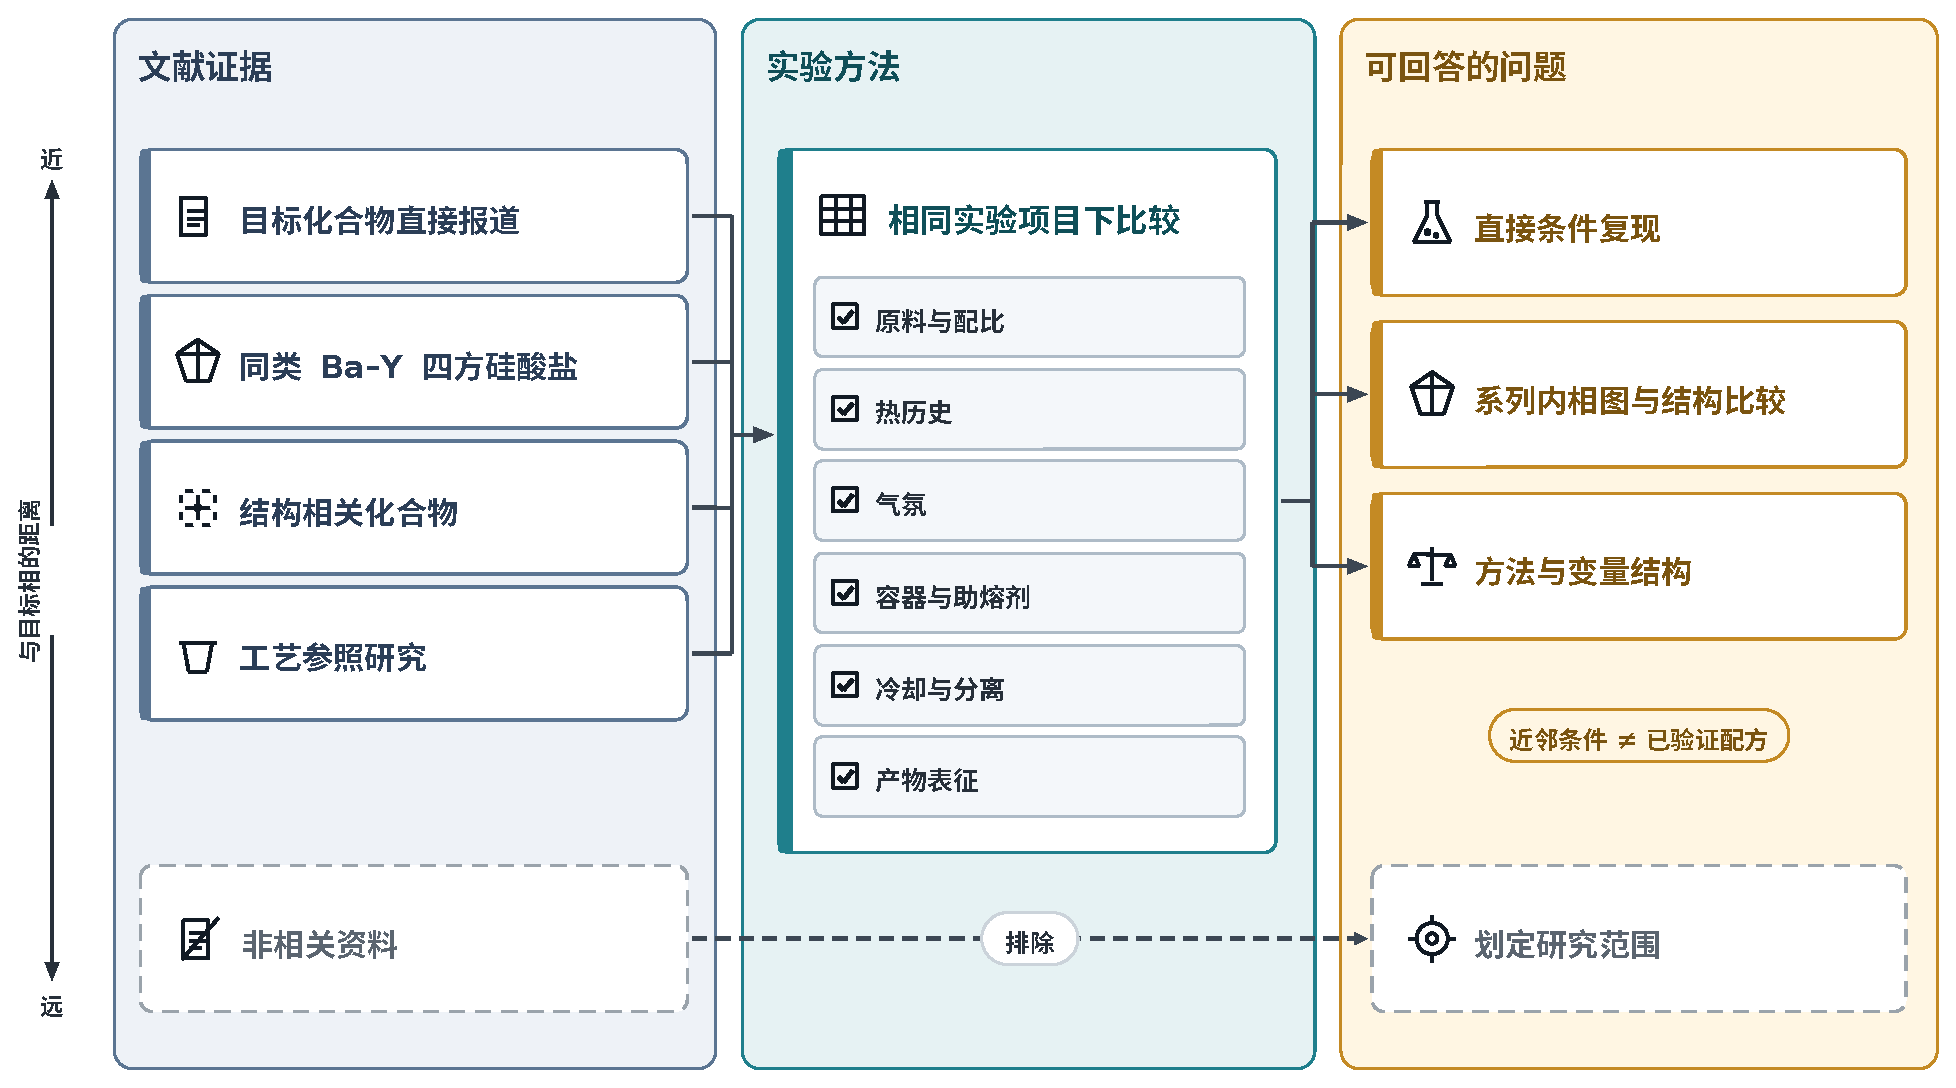
\includegraphics[width=\linewidth]{../figures/pdf/fig01_evidence_synthesis_map.pdf}
  \caption[不同文献对目标化合物合成研究的适用范围]{\textbf{不同文献对目标化合物合成研究的适用范围。}左侧依次列出目标化合物直接报道、同类Ba--Y四方硅酸盐、结构相关化合物、工艺参照研究和非相关资料；中部按相同实验项目整理原料、热历史、气氛、容器、冷却和产物表征；右侧说明各类资料所能明确的问题。目标化合物的直接报道目前仅有一篇\cite{ababaikeri2024ba5y12zn}。相关体系的数值仅用于说明实验变量和表征方法，不能直接作为目标相的已验证配方。}
  \label{fig:evidence-map}
\end{figure}

图~\ref{fig:evidence-map}\CJKecglue{}给出文献对象、实验条件与所能明确的问题之间的对应关系。比较时先确认文献实际研究的相，再在相同实验项目下比较原料、热历史、气氛、容器和冷却条件。这种整理便于比较，但不消除化合物之间的结构差异。文献与目标相的关系越远，可借鉴的内容越限于变量设置、实验设计和表征方法，具体温度、配比或助熔剂用量不能直接移用。

\subsection{结构相关性}

结构相关性至少要求有可追溯的晶体学证据，不能仅依据元素组相形成同。Ba$M$SiO$_4$（$M$~=~Co、Zn、Mg）经单晶X射线衍射和粉末中子衍射归入填充鳞石英（stuffed-tridymite）衍生结构族\cite{liu1993structures}。该结果可用于比较Zn、Mg和Co的四面体网络，但该结构族不含Y且结构系列不同，不能作为目标相的直接依据。BaZn$_2$Si$_2$O$_7$的低温结构与高温结构经中子衍射和X射线衍射区分\cite{lin1999phase}；Ba$_2$ZnSi$_2$O$_7$的单斜结构由单晶精修确立\cite{kaiser2002crystal}；BaZnSi$_3$O$_8$的衍射结果给出了ZnO$_4$与SiO$_4$的连接网络\cite{zou2021crystal}。这些研究有助于确定待比较的结构参数，但不能确定目标相在何种条件下可复现。

Ba--Si--O体系中四配位Si网络的复杂性及其热响应仅可作为间接的结构参照\cite{gorelova2016thermal}。Y$_2$Si$_2$O$_7$的多晶型及其热膨胀数据表明，同一组成可对应不同结构，跨年代比较须核对结构模型和观测温度\cite{dolan2008structures,becerro2004revision}。这些结果可用于提出结构表征问题，但不提供目标相的稳定区间。

综上，同类Ba--Y硅酸盐研究可用于检验组成和相区，结构相关研究可用于比较位点和表征方法，工艺参照研究可用于完善实验设计。具体合成条件只能在原始研究对象和实验范围内解释，不能因化合物“相似”而直接外推。

\subsection{非相关资料的界定}

仅含Ba和Si不足以构成结构相关性。蓝锥矿（benitoite）型BaSi$_4$O$_9$的结构精修\cite{finger1995refinement}、高压BaSi$_4$O$_9$的三方结构\cite{hazen1999crystal}、硅酸三钡（tribarium silicate）的结构精修\cite{tillmanns1978refinement}以及高温Ba$_2$[Si$_4$O$_{10}$]的结构报道\cite{katscher1973the}均表明，Ba--Si--O网络可具有不同结构，但缺少目标相所需的Y\slash Zn位点对应关系。高压Ba硅酸盐中出现9R/6H钙钛矿型结构的报道进一步表明，压力路径可能通向另一类网络，不能据此反推常压下的目标路线\cite{yusa2007rhombohedral}。

同样，应用背景相近也不能替代结构证据。Ce$^{3+}$掺杂Ba$_5$Si$_8$O$_{21}$的光学研究未提供Y\slash Zn目标相的归属信息\cite{zhong2020combining}；非中心对称LiBa$_2$GaSi$_2$O$_8$与目标相仅在光学应用背景上相近，组成和结构系列均不相同\cite{gu2025liba2gasi2o8}。填充型硅石结构（stuffed silica）的经典概念以及零热膨胀材料的理论--实验综述有助于统一术语和理解热机械行为，但不能支持目标相的配方判断\cite{buerger1954the,erlebach2020thermomechanical}。

因此，非相关资料仅用于划定研究范围，不进入目标相的合成条件比较。即使将相关资料列于同一表中，也仅表示实验项目可比较，不表示不同化合物具有相同的结构或相形成条件。
